Comparison between the global biophysical features (Fig. \ref{fig:global_biophysical}) 
shows that periplasmic proteins have an higher tendency toward sheet and coil formation,
but lower tendency towards helix formation when compared to cytoplasmic proteins. 
In addition, they show more sidechain and backbone dynamics,
and a decreased tendency towards early folding.

~\begin{figure}[h!]
	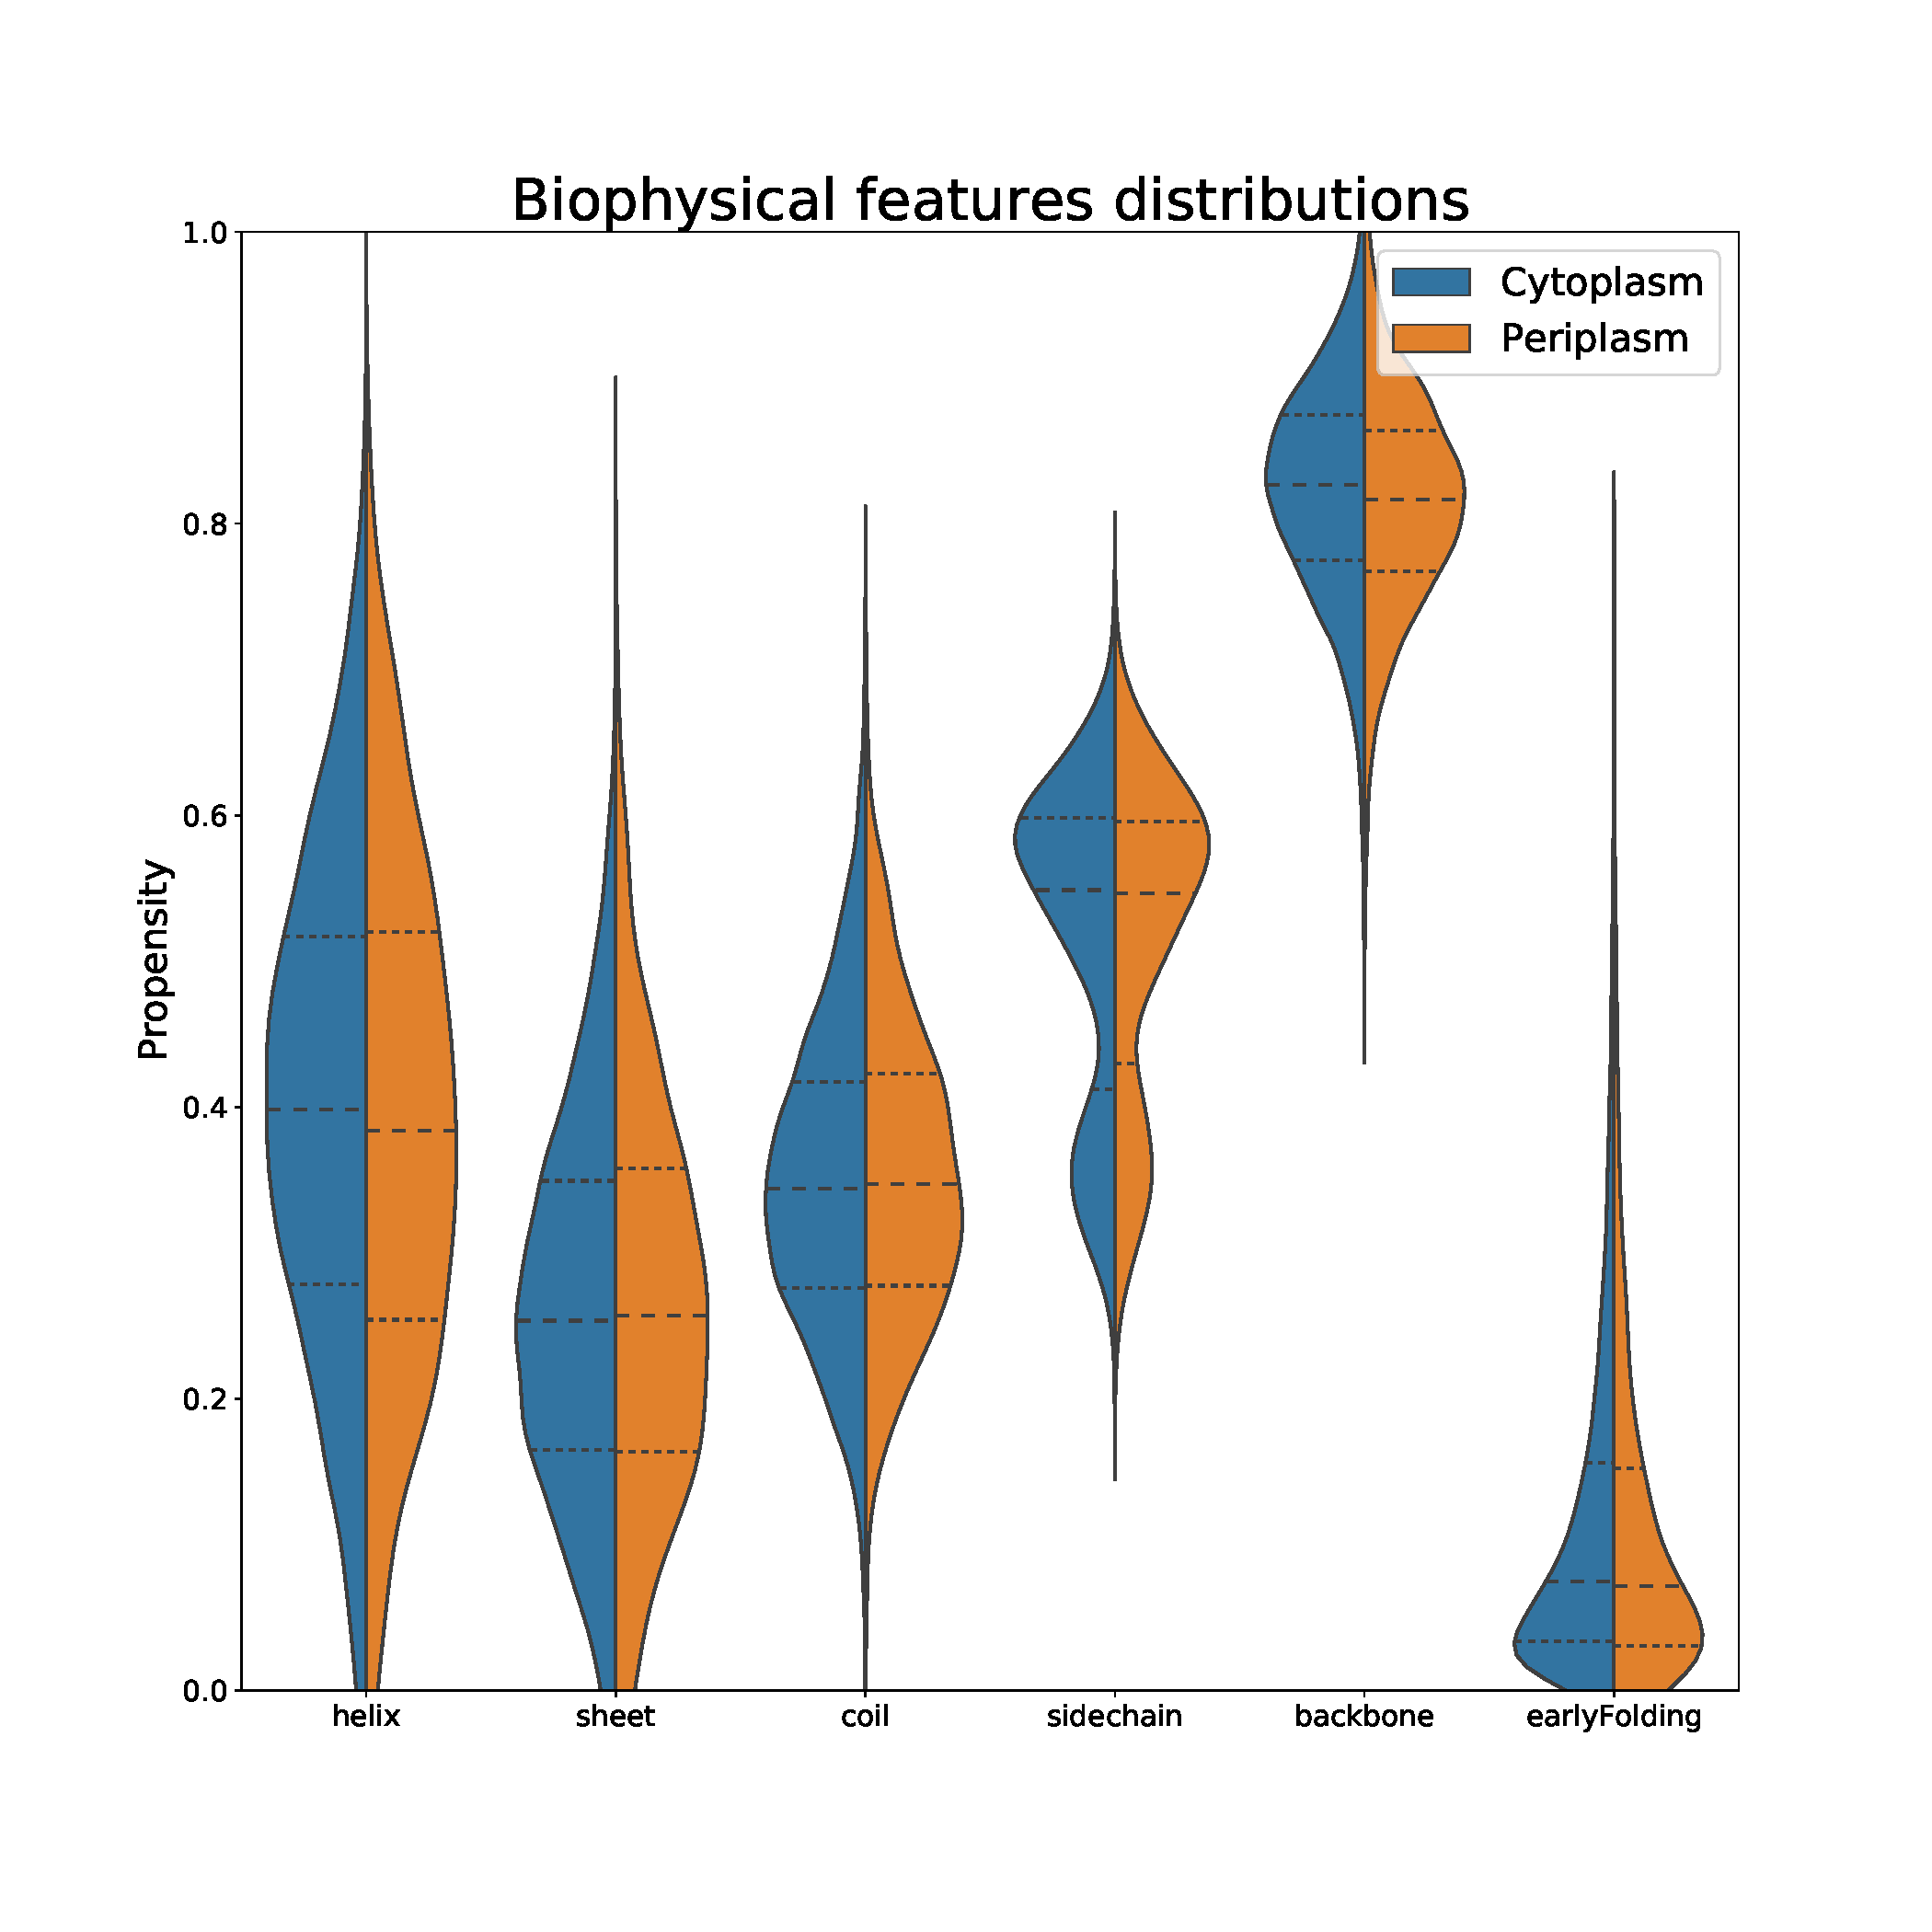
\includegraphics[width=\linewidth]{./results/general_comparison/global_comparison/biophysical/img/features_violin.pdf}
	\caption{
		\textbf{Comparison between the biophysical propensity distributions of cytoplasmic and periplasmic proteins.}
		Propensities toward 
		\textit{helix,
		sheet,
		coil,
		sidechain,
		backbone,}
		and
		\textit{earlyFolding}
		were predicted by EFoldMine and DynaMine.
		In total there were 11,424,793 residues (each with a predicted propensity toward the biophysical features described above) spread over 30,632 cytoplasmic  and 3,883 periplasmic proteins.
		In general, the distribution have a similar shape,
		but differences are significant, P-value determined by the Wilcoxon-ranksum test.
		Periplasmic as compared to cytoplasmic proteins tend to have
		less propensity toward helical formation (P-value 0.0),	
		but increased propensity toward sheet (P-value 4e-57) and coil (P-value 9e-252) formation.
		They have an increased sidechain (P-value 2e-9) and backbone (P-value 0.0) dynamics,
		and a decreased propensity toward early folding (P-value 0.0).
		}
	\label{fig:global_biophysical}
~\end{figure}
